\subsection*{Disjoint Sets}
Earlier in this section, we discussed the concept of set equality and the relation of one set being a subset of another set.  There are other possible relationships between two sets; one is that the sets are disjoint.  Basically, two sets are disjoint if and only if they have nothing in common.  We express this formally in the following definition.
%
\begin{defbox}{D:disjointsets}{Let  $A$  and  $B$  be subsets of the universal set  $U$.  The sets  $A$  and  $B$  are said to be \textbf{disjoint}
\index{disjoint}%
\index{disjoint sets}%
 provided that  $A \cap B = \emptyset $.}
\end{defbox}
%
For example, the Venn diagram in Figure~\ref{fig:asubsetb2} shows two sets  $A$  and  $B$  with  
$A \subseteq B$.  The shaded region is the region that represents $B^c$.
%
\begin{figure}[h]
\begin{center}
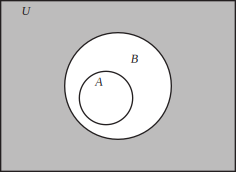
\includegraphics{figps-asubsetb2.eps}
\caption{Venn Diagram with $A \subseteq B$} \label{fig:asubsetb2}
\end{center}
\end{figure}
From the Venn diagram, it appears that  $A \cap B^c  = \emptyset $.  This means that  $A$  and  $B^c$  are disjoint.
%
The preceding example suggests that the following proposition is true:
\begin{center}
If  $A \subseteq B$, then  $A \cap B^c  = \emptyset $.
\end{center}
If we would like to prove this proposition, a reasonable ``backward question'' is, ``How do we prove that a set $\left( \text{namely } A \cap B^c \right)$ is equal to the empty set?''

This question seems difficult to answer since how do we prove that a set is empty?   This is an instance where proving the contrapositive or using a proof by contradiction could be reasonable approaches.  To illustrate these methods, let us assume the proposition we are trying to prove is of the following form:
\begin{center}
If  $P$, then  $T = \emptyset $.
\end{center}
If we choose to prove the contrapositive or use a proof  by contradiction, we will assume that  
$T \ne \emptyset $.  These methods can be outlined as follows:
\begin{itemize}
\item The contrapositive of ``If  $P$, then  $T = \emptyset $'' is, ``If $T \ne \emptyset $, then $\mynot P$.''  So in this case, we would assume  $T \ne \emptyset $ and try to prove $\mynot P$.

\item Using a proof by contradiction, we would assume $P$ and assume that  $T \ne \emptyset$.  From these two assumptions, we would attempt to derive a contradiction.

\end{itemize}
One advantage of these methods is that when we assume that  $T \ne \emptyset $, then we know that there exists an element in the set  $T$.  We can then use that element in the rest of the proof.  We will prove one of the conditional statements for Proposition~\ref{P:subsetprop} by proving its contrapositive.  The proof of the other conditional statement associated with Proposition~\ref{P:subsetprop} is Exercise~(\ref{exer:subsetprop}).
%\hbreak
\begin{proposition} \label{P:subsetprop}
Let $A$  and  $B$  be subsets of some universal set.    Then $A \subseteq B$ if and only if 
$A \cap B^c  = \emptyset $.
\end{proposition}
%
\begin{myproof}
Let  $A$  and  $B$  be subsets of some universal set.  We will first prove that if  $A \subseteq B$, then  $A \cap B^c  = \emptyset $, by proving its contrapositive.  That is, we will prove
\begin{center}
If   $A \cap B^c  \ne \emptyset $, then  $A \not \subseteq B$.
\end{center}
So assume that  $A \cap B^c  \ne \emptyset $.  We will prove that  $A \not \subseteq B$ by proving that there must exist an element  $x$  such that  $x \in A$  and  $x \notin B$.

Since  $A \cap B^c  \ne \emptyset $, there exists an element  $x$  that is in  $A \cap B^c $.  This means that
\[
x \in A\text{  and  }x \in B^c. 
\]
Now, the fact that  $x \in B^c $ means that  $x \notin B$.  Hence, we can conclude that
\[
x \in A\text{  and  }x \notin B.
\]
This means that  $A \not \subseteq B$, and hence, we have proved that if $A \cap B^c  \ne \emptyset $, then  
$A \not \subseteq B$, and therefore, we have proved that if $A \subseteq B$, then  $A \cap B^c  = \emptyset$.

The proof that if $A \cap B^c = \emptyset$, then $A \subseteq B$ is Exercise~(\ref{exer:subsetprop}).
\end{myproof}
\hbreak


\begin{prog}[\textbf{Proving Two Sets Are Disjoint}] \label{prog:disjointsets} \hfill \\
It has been noted that it is often possible to prove that two sets are disjoint by using a proof by contradiction.  In this case, we assume that the two sets are not disjoint and hence, their intersection is not empty.  Use this method to prove that the following two sets are disjoint.
\[
A = \{ x \in \Z \mid \mod{x}{3}{12} \} \quad \text{and} \quad B = \{ y \in \Z \mid \mod{y}{2}{8} \}.
\]
\end{prog}
\hbreak


\subsection*{A Final Comment}
We have used the choose-an-element method
\index{choose-an-element method}%
 to prove Propositions~\ref{P:SissubsetT}, \ref{P:setdifference}, \linebreak 
and~\ref{P:subsetprop}.  Proofs involving sets that use this method are sometimes referred to as \textbf{element-chasing proofs.}
\index{element-chasing proof}%
\index{proof!element-chasing}%
  This name is used since the basic method is to choose an arbitrary element from one set and ``chase it'' until you prove it must be in another set.
\hbreak

\endinput
